\section{Angular}

\subsection{Allgemeines [M]}
\setauthor{Fabian Maar}
Angular ist ein Framework für Webapplikation, das auf der Programmiersprache Typescript basiert. Es ist eines der renommiertesten Frameworks zur Front-End-Entwicklung und wird als Open-Source-Software zur Verfügung gestellt. Besonders bietet sich Angular für Single-Page-Webanwendung an, da es ein komponentenbasiertes Framework ist. Das bedeutet, der Code ist wiederverwendbar und verkapselt. Komplexe Logiken werden auf ihre Grundelemente reduziert und beeinflussen sich nicht gegenseitig. 

\subsection{Dependency [L ]}
\setauthor{Litzlbauer Lorenz}
Um eine nachvollziehbare Auswahl zu treffen, muss verstanden werden, wie Angular
funktioniert. In den folgenden Unterabschnitten wird sich mit den Technologien auf die Angular aufgebaut ist, auseinandergesetzt. 

\subsubsection{RxJS}
\setauthor{Litzlbauer Lorenz}
ReactiveX ist eine Library für das Erstellen von asynchronen und Event-basierenden Programmen, dafür benutzt es  \emph{observable sequences}.
Die Library erweitert so, dass \emph{Observer-Design-Pattern} mit verschiedenen neuen Operatoren und händelt dabei "Lowlevel"-Funktionen wie Threading, Synchronisation, Thread-Sicherheit und das nicht-blockieren von I/O vergleiche \cite{ReactiveXIntro}

RxJS ist eine Implementierung von ReactiveX für die Programmiersprache Javascript. Angular verwendet RxJS für reaktive Programmierart.
\subsubsection{Webpack}
\setauthor{Litzlbauer Lorenz}
Die Hauptfunktion von Webpack ist es, viele verschiedenen Daten zu einem Paket für eine JavaScript Applikation zusammenzufassen, dabei optimiert es die Dateigröße, indem es mithilfe von einem selbst generierten \emph{dependency-graph} die Abhängigkeiten der Applikation überprüft und nur notwendige Teile für die JavaScript-Applikation der Daten nimmt. Bei der Zusammenfassung werden Sprachen, die der Webbrowser nicht Interpretieren kann wie Typescript, Sass uvm. in die für den Webbrowser verständlichen Gegenstücke gewandelt. Webpack hat aber auch viele andere Features. Vergleiche \cite{Webpack}
\setauthor{Litzlbauer Lorenz}
Angular benutzt Webpack um TypeScript in JavaScript und Sass bzw. Scss in Scss zu wandeln, um beim Bauen des Projektes alle Module in ein einziges zusammenzufassen und um die Applikation bei der Entwicklung zu \emph{Live-Reloading} zu unterstützen. Dabei wird bei einer Änderung im Code die gesamte Applikation geupdatet und neu gestartet. 

\subsection{Vorteile/Auswahlkriterien [M]}
\setauthor{Fabian Maar}
Dieses komponentenbasierte Programmieren war eines der vielen Gründe 
warum Angular die beste Option ist. Im Abschnitt 5 //TODO  wird nochmals deutlich, wie dieser Aspekt genutzt wird. Ein weiterer Grund, ist die einfache Einbindung von 
Libraries und deren Übersichtlichkeit, die durch ngModules ermöglicht werden. Die ständige Erweiterung und die Unterstützung von Third-Party-Libraries, die unter anderem für die 3D-Darstellung verwendet werden, wird ebenfalls von diesen ngModulen ermöglicht. 
Beispiele wie wir dieses ngModule aufgesetzt haben befinden sich im Abschnitt Landing-Page aufsetzen //TODO VERLINKEN. Auch aufgrund von persönlichen Erfahrungen im Unterricht und in anderen Projekten war Angular die beste Auswahlmöglichkeit.

\section{Webstorm}
\setauthor{Fabian Maar}
Webstorm ist eine Entwicklungsumgebung vom Unternehmen JetBrains, die sich auf die Programmiersprache JavaScript spezialisiert hat. Ebenfalls unterstützt es besonders Frameworks wie Angular. Das Webstorm besonders auf Angular optimiert wurde, zeigt sich durch viele Features, die das Entwickeln von Angular-Projekten erleichtern. So macht es Webstorm möglich, mit nur wenigen Mausklicks eine neue Angular-Dependency oder Komponente zu erstellen. Auch wird die Entwicklungszeit durch intelligente Code-Vervollständigung, Code-Formatierung, einfache Navigation und viele weitere hilfreiche Features deutlich verkürzt. 

\section{ThreeJs [L]}
\setauthor{Litzlbauer Lorenz}
\begin{wrapfigure}{r}{0.3\textwidth}
    \begin{center}
      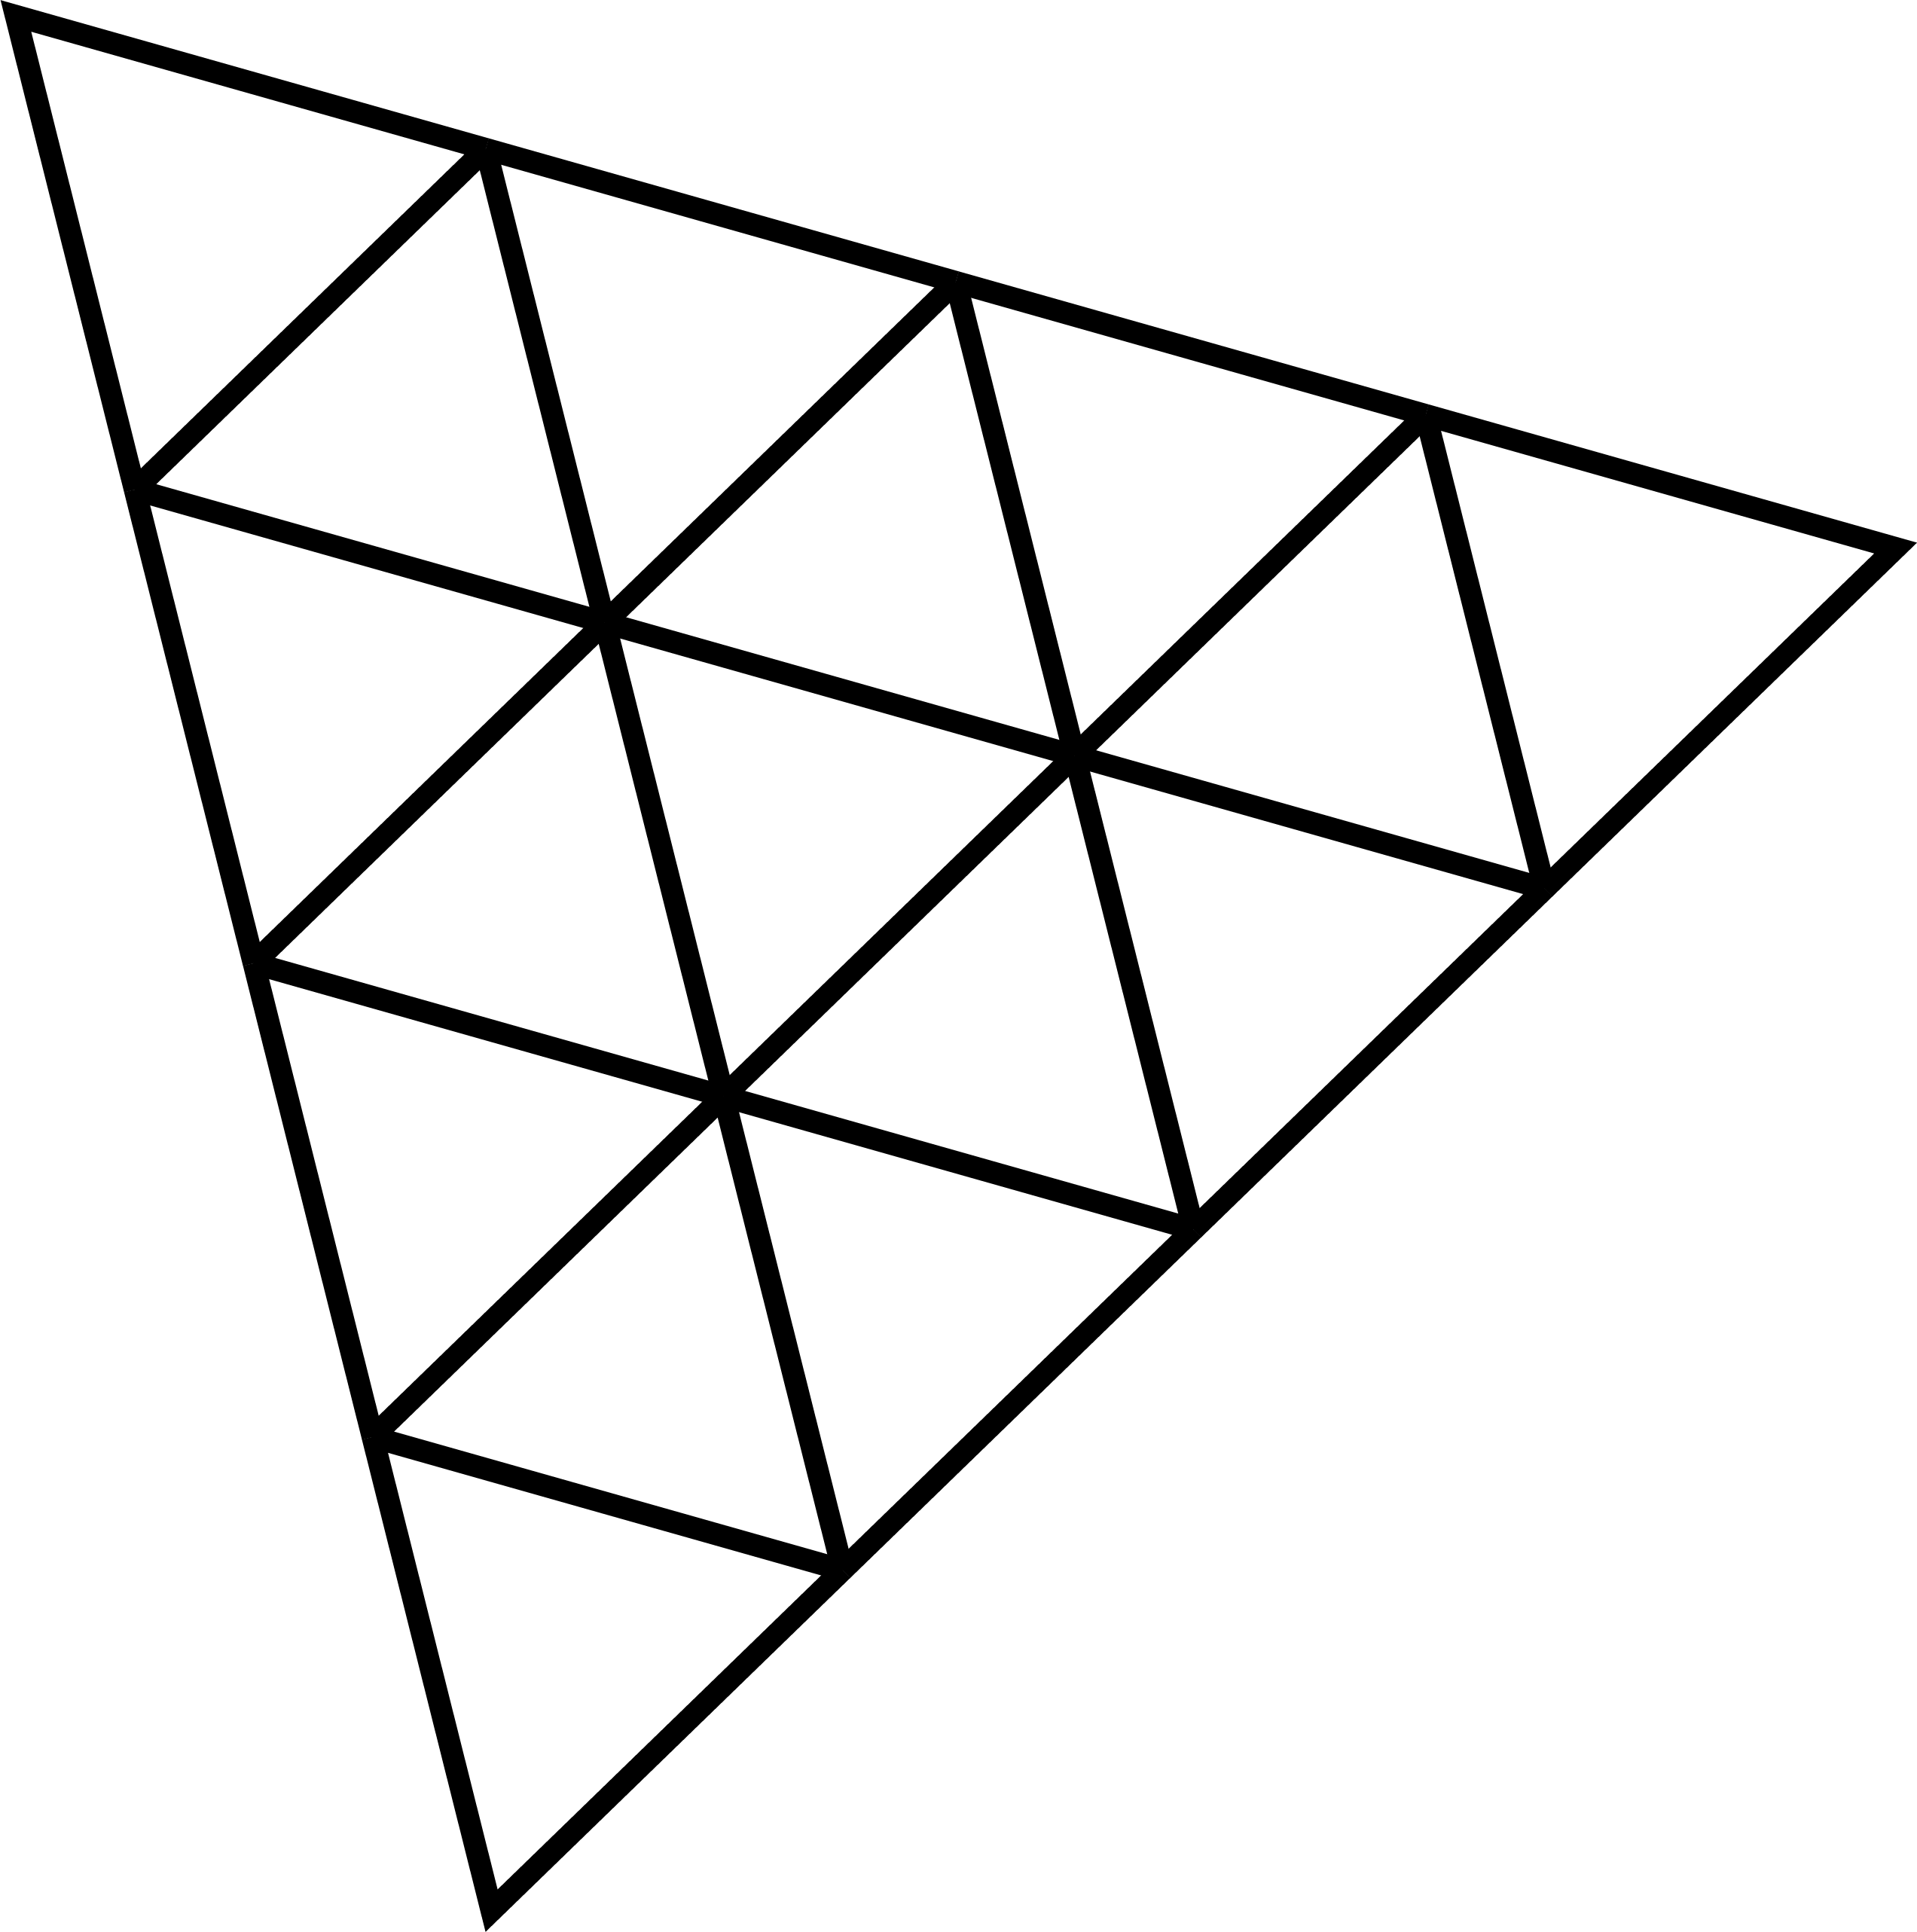
\includegraphics[width=0.2\textwidth]{pics/threeJS.png}
     \caption{ThreeJs Logo}
    \end{center}
\end{wrapfigure}
ThreeJs ist eine JavaScript Library für die Darstellung von 3D-Grafiken im Web. Für die 3D-Darstellung nutzt ThreeJs meistens WebGL (mehr dazu im nächsten Abschnitt \hyperref[ch::ThreeJsDependency]{ThreeJs Dependency}), ein low-level Framework. WebGl hat eine hohe Komplexität. ThreeJs bietet eine Abstraktion, bei der es viele Sachen wie die 3D-Szene, Lichter, Schatten, Materialien, Texturen und 3D-Mathe händelt, um die 3D-Darstellungen im Web einfacher zu gestalten. In ThreeJs werden Geometrie, Objekte und Materialien verbunden, um ein 3D-Objekt zu erstellen. Dabei kann die Struktur einer Szene der Abbildung \ref{fig:tech:front:threejsstructure} ähneln. Vergleiche \cite[ThreeJs fundamentals]{ThreeJsFund}

\begin{figure} [h t]
    \centering
    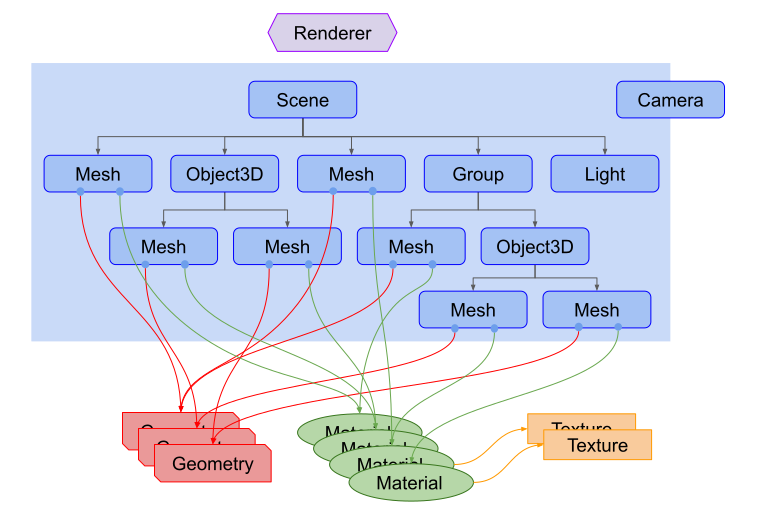
\includegraphics[scale=0.5]{pics/threejs-structure.png}
    \caption{Die Struktur von ThreeJs}
    \label{fig:tech:front:threejsstructure}
\end{figure}

\subsection{Dependency}
\label{ch::ThreeJsDependency}
Um einen Großteil der 3D-Darstellungen zu rendern, benutzt ThreeJs WebGL.

\subsubsection{WebGL}
\label{ch::webgl}
\begin{wrapfigure}{h  r}{0.3\textwidth}
    \begin{center}
      
\includegraphics[width=0.2\textwidth]{pics/WebGL_Logo.png}
     \caption{ThreeJs Logo}
    \end{center}
\end{wrapfigure}
WebGl ist eine lizensfreie Api, die dafür benutzt wird 3D-Grafiken im Web darzustellen. Sie basiert auf OpenGL ES 2.0 und benutzt auch dieselbe shading language GLSL. WebGL ist eine Low-Level-API, das bedeutet, dass schon sehr einfache Projekte einen hohen Programmieranteil haben. Vergleiche\cite[WebGl Getting Started]{WebglGettingStarted}


\subsection{Auswahlkriterien}
Es gab verschiedene Auswahlkriterien für die 3D-Web-API.
\begin{compactitem}
  \item Effizienzen der 3D Engine (Hardware Acceleration, RAM-Auslastung)
  \item Benutzerfreundlichkeit (Programmerexperience)
  \item Zusätzliche Features
  \item Die Features des Projektes müssen damit umsetzbar sein
  \begin{compactenum}
    \item Das Laden von 3D-Modellen aus 3D-Dateinen und aus dem Internet
    \item Video-Texturen support
  \end{compactenum}
\end{compactitem}

\subsubsection{Alternativen 3D Web Apis}
Es gibt viele Technologien, die 3D-Grafiken im Web ermöglichen, wie Three.js, Babylon.js, A-Frame, X3DOM und WebGL

\paragraph{A-Frame}
A-Frame wird von der Morzilla Foundation als OpenSource-Projekt entwickelt. Die 3D-Szene wird durch eine deklarative Sprache mit XML-Syntax definiert. Über die WebVR-API bietet die Libray auch die Möglichkeit, die 3D-Szenen durch eine VR-Brille zu erfahren. Bei der 3D-Darstellung setzt A-Frame auf ThreeJs. \cite[A-Frame Wikipedia]{a-frame-wiki}

A-Frame hat ähnliche Funktionen und Leistung im Vergleich zu ThreeJs, da es ja schlussendlich darauf aufbaut. A-Frame sticht bei der VR support hervor (ThreeJs hätte auch eine Unterstützung dafür, diese ist aber schwieriger einzubinden), doch ist das kein unbedingt nötiges Feature. ThreeJs ist ja bereits eine Abstraktion von WebGL. Für das Projekt wird keine weiter Abstraktion gebraucht.

\paragraph{WebGL}
Im Vorherigen Kapitel wurde sich bereits mit WebGL befasst. \ref{ch::webgl}
Um nur eine einfache 3D-Szene in WebGL darzustellen, muss sehr viel Code geschrieben werden. Denn WebGL übernimmt keine Low-Level-Funktion. Es müssen Matrixrechnungen für die Transformationen von 3D-Objekt Manuel und Vertex buffers, die die Daten der Vertex Positionen, Normaldaten, Farben und Texturen, selbst programmiert werden und das in einer eigenen Programmiersprache. Deshalb war WebGL keine Option für das Projekt.

\subsubsection{Angular Three}
Angular Three ist ein Open Source Projekt von Matt DesLauriers. Es zielt darauf ab die Vorteile von Angular und ThreeJs zu kombinieren. Dabei verbindet es das Prinzip der Komponenten von Angular mit der 3D Darstellung von ThreeJs. 

\begin{lstlisting}[language=html,caption=Angular Three - Komponentenbasiertes 3D Scenen in HTML,label=lst:impl:AngularThreeExampleCode]
<ngt-canvas>
    <ngt-ambient-light intensity="0.5"></ngt-ambient-light>
    <ngt-spot-light [position]="10" angle="0.15" penumbra="1"></ngt-spot-light>
    <ngt-point-light [position]="-10"></ngt-point-light>
  
    <app-cube [position]="[1.2, 0, 0]"></app-cube>
    <app-cube [position]="[-1.2, 0, 0]"></app-cube>
  
    <ngt-soba-orbit-controls></ngt-soba-orbit-controls>
</ngt-canvas>
\end{lstlisting}

\begin{lstlisting}[language=html,caption=Angular Three - App Cube,label=lst:impl:AngularThreeCube]
<ngt-mesh
  (beforeRender)="onCubeBeforeRender($event)"
  (click)="active = !active"
  (pointerover)="hovered = true"
  (pointerout)="hovered = false"
  [scale]="active ? 1.5 : 1"
  [position]="position"
>
  <ngt-box-geometry></ngt-box-geometry>
  <ngt-mesh-standard-material [color]="hovered ? 'turquoise' : 'tomato'"></ngt-mesh-standard-material>
</ngt-mesh>
\end{lstlisting}
Ein Vorteil von Angular Three ist, dass durch nur wenige Zeilen Code \ref{lst:impl:AngularThreeExampleCode} eine 3D-Szene mit Lichtern und Orientierungsfunktionen erstellt werden kann und die Business-Logik, App-Cube \ref{lst:impl:AngularThreeCube} durch die Verwendung einer Komponente ausgelagert werden kann.

Ein weiterer Vorteil von Angular Three ist die ausführliche Dokumentation mit Codebeispielen. \href{https://angular-three.netlify.app/docs/getting-started/overview}{(link) Angular Three Dokumentation https://angular-three.netlify.app/docs/getting-started/overview}

Wegen der vielen Vorteile hohe Benutzerfreundlichkeit, ähnliche 3D-Leistung zu ThreeJs (Angular Three basiert auf ThreeJs, welches selbst die WebGL-Renderengine benutzt) und wegen der Verbindung von Angular und ThreeJs Features bietet sich die Liberay für das Projekt an.

Mithilfe eines Prototypen ( mehr dazu im Abschnitt \hyperref[ch::ongoing-prototyping]{fortlaufendes Prototyping} ) wurde getestet, ob Angular Three alle Features, die für das Projekt benötigt werden, unterstützen kann, die für das Projekt nötig sind. Dabei wurde festgestellt, dass sich die Liberay Angular für das Projekt nicht eignet. Denn beim Prototyping sind Fehler aufgetreten. Beim erneuten Laden von 3D-Objekten aus derselben Datei haben sich keine Daten mehr im Objekt befunden. ThreeJs Module funktionierten Teilweise nicht, wie die FristPersonControls. 

Weil Angular Three nicht die für das Projekt aufgestellten Anforderungen erfüllt hat, wurde der Prototyp zu ThreeJs migriert, weil sich die Syntax ähnelt und dadurch nur wenig Aufwand bei der Migrierung entstand. Diese 3D-Library wurde schlussendlich auch im Projekt verwendet.